\documentclass[tikz,border=2pt]{standalone}
\usepackage{amsmath}
\usepackage{pgfplots}
\pgfplotsset{compat=1.18}
\usetikzlibrary{arrows.meta}
\begin{document}
% Example 2 (Exercise 3.1): V2 = {-x1+x2<=2, -2x1-x2<=-8, -x1-x2<=-5}; pairs of boundary lines meet at (2,4) and (3,2),
% which lie in V2 and are its extreme points, and at (3/2,7/2), which violates -2x1-x2<=-8.
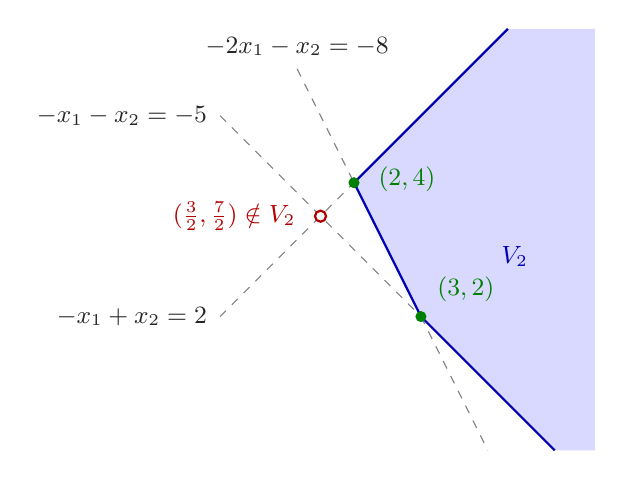
\begin{tikzpicture}[font=\small, >={Latex[length=2mm]}]
  \begin{scope}[x=0.85cm, y=0.85cm]
    \fill[blue!15] (2,4) -- (4.3,6.3) -- (5.6,6.3) -- (5.6,0) -- (5,0) -- (3,2) -- cycle;
    \draw[gray, thin, dashed] (0,2) -- (2,4);
    \draw[gray, thin, dashed] (1.15,5.7) -- (2,4) (3,2) -- (4,0);
    \draw[gray, thin, dashed] (0,5) -- (3,2);
    \draw[blue!70!black, thick] (4.3,6.3) -- (2,4) -- (3,2) -- (5,0);
    \fill[green!50!black] (2,4) circle (2pt) (3,2) circle (2pt);
    \draw[red!70!black, thick, fill=white] (1.5,3.5) circle (2pt);
    \node[green!50!black, anchor=west] at (2.22,4.05) {$(2,4)$};
    \node[green!50!black, anchor=south west] at (3.1,2.08) {$(3,2)$};
    \node[red!70!black, anchor=east] at (1.27,3.5) {$(\tfrac{3}{2},\tfrac{7}{2})\notin V_2$};
    \node[blue!70!black] at (4.4,2.9) {$V_2$};
    \node[gray!30!black, anchor=east] at (-0.05,2) {$-x_1+x_2=2$};
    \node[gray!30!black, anchor=south] at (1.15,5.75) {$-2x_1-x_2=-8$};
    \node[gray!30!black, anchor=east] at (-0.05,5) {$-x_1-x_2=-5$};
  \end{scope}
\end{tikzpicture}
\end{document}
